\documentclass[./main.tex]{subfiles}

\begin{document}
\section{Improving the Model}\label{sec:improving}
In the following section we will use our knowledge about the developed model to modify and improve the performance of the Stacked hourglass. We will start off in Section \ref{subsec:improv_motivation}, where we will be giving a brief overview of how the model will be improved. Then, in Section \ref{subsec:improv_conf_details} the configuration details of the model will be explained and argued for. Section \ref{sec:improv_results} then presents the results of the modified model. Lastly, in Section \ref{subsec:improv_train} the various training details will be described.

\subsection{Motivation}\label{subsec:improv_motivation}
In Section \ref{sec:XAI} we explored the developed model from Section \ref{experiement}. By doing so we found out, that the latent space of the model has some inconsistency of the placement of the training observations, as well as having some principal components that act as noise, which could explain the not optimal performance of the model. By helping improving the latent space of the model, as well as removing some of the noise, we could improve the performance of the model, which can be done by making use of an autoencoder.

\subsection{Configuration Details}\label{subsec:improv_conf_details}
\begin{figure}[htbp]
    \centering
    
\includegraphics[width = \textwidth - 1 cm]{entities/Ae_model.png}
    \caption{Visualization of the architecture of the developed autoencoder. The numbers in each box represents the dimensions of the output of the corresponding layer.}
    \label{fig:AE_model}
\end{figure}
\noindent The developed autoencoder is visualized in Figure \ref{fig:AE_model}. The autoencoder makes use of convolutional layers and a linear layer to downsample the input down to only $50$ dimensions. We chose $50$ as the dimensions of the bottleneck, as we saw in Section \ref{subsec:shape_analysis}, that principal component $50$ and above act as noise, indicating that we need $50$ or less dimensions. The autoencoder uses an decoder that is identical to the encoder, however flipped, to produce the final predictions. 
\\
\\
The input of the autoencoder has the dimensions of $256 \times 4 \times 4$. As the width and height of the input already has a size of only $4 \times 4$, it does not make sense to use max pooling or similar methods to reduce this. Instead, the autoencoder only reduces the $256$ layers of the input. This is done by making use of convolutional layers, that should learn the best way to reduce the amount of layers in the data.  The innermost layers use linear layers instead of convolutional layers, as they make it easier to control the dimensions of the latent space, compared to the case with convolutional layers. We decided to use ReLU as the acitvation function of the autoencoder, as ReLU has some advantages, which we described in Section \ref{subsec:general_ML_terminology}, as well as it makes the autoencoder be in the same range as the Stacked Hourglass.
\\
\begin{figure}[htbp]
    \centering
    
\includegraphics[width = \textwidth - 1 cm]{entities/SHG_AE.png}
    \caption{Visualization of the proposed combination of the hourglass and autoencoder for the Stacked hourglass.}
    \label{fig:SHG_AE}
\end{figure}
\\
The autoencoder takes the output of the third residual of the bottleneck of our developed Stacked hourglass as input, hence why the autoencoder will be placed after the third residual to form a new proposed hourglass for the Stacked hourglass, as visualized in Figure \ref{fig:SHG_AE}.
\\
\\
The training of the new model consits of two parts to speed up the training. First the autoencoder is trained isolated. Then, the trained autoencoder is placed in the developed Stacked hourglass, following the structure of Figure \ref{fig:SHG_AE}, and the whole network is trained.
\\
\\
The autoencoder is trained using stochastic gradient descent with momentum with $\alpha = 0.9$ and $\bm{v} = \bm{0}$, $MSE$ as the loss function, a learning rate of $5e-4$, which is halved every $25$th epoch, and a mini-batch size of $16$. To increase the robustness of the autoencoder, we add noise sampled from
$$\mathcal{N} \left(0, x^2e-2 \right)$$
to each input training sample, where $x$ is the value of the training sample. To help the model converge, we initialize all parameters by sampling from a Glorot normal distribution, like in the case with the Stacked hourglass.
\\
\\
After the autoencoder has been trained it is placed in the hourglass of the developed Stacked hourglass. The modified Stacked hourglass is then trained by following Newell \textit{et al.} \cite{Newell} as described in Section \ref{subsec:conf_details}.
\begin{figure}[htbp]
    \centering
    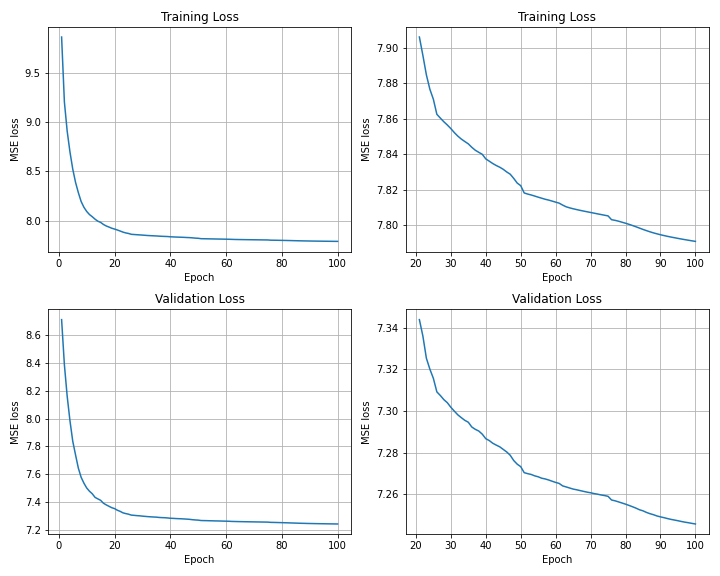
\includegraphics[height = 8 cm]{entities/AE_evolution.png}
    \caption{Visualization of the evolution of the training- and validation loss of the autoencoder during training. The left column shows all of the $100$ epochs. Right column shows epoch $21$ and foward}
    \label{fig:AE_evolution}
\end{figure}

\subsection{Results}\label{sec:improv_results}
\begin{figure}[htbp]
    \centering
    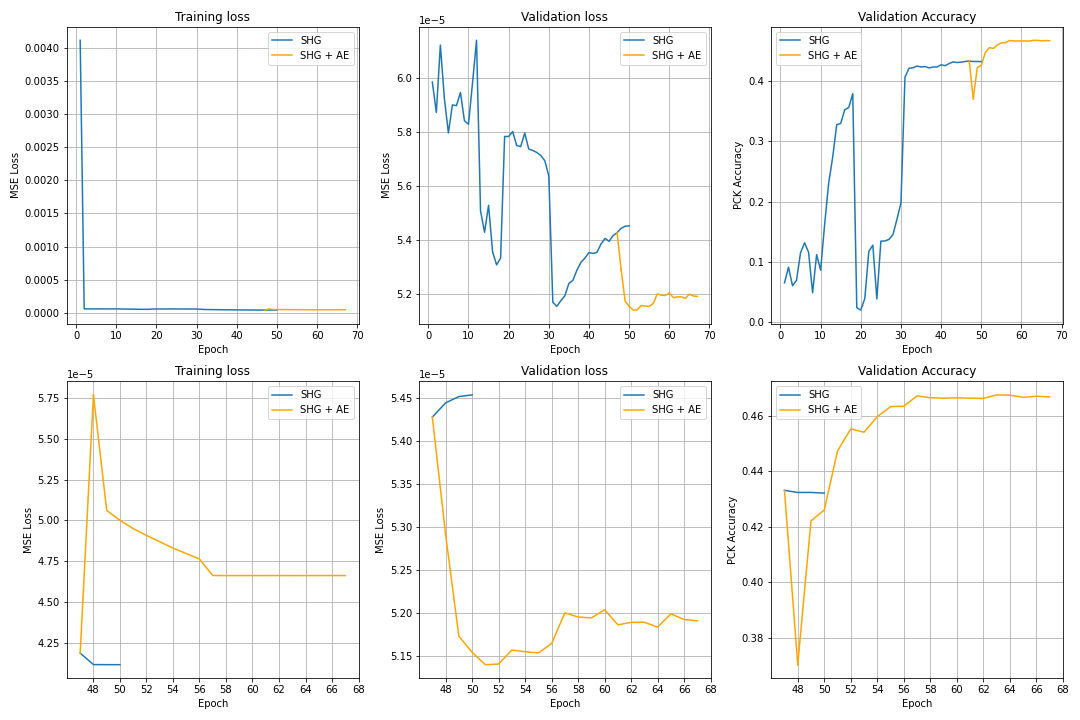
\includegraphics[width = \textwidth - 1 cm]{entities//SHG_AE_Evolution.png}
    \caption{Visualization of the evolution of the training- and validation loss, as well as the PCK validation accuracy of the combination of the Stacked hourglass and autoencoder, compared with the evolution of training the orignial Stacked hourglass. The top row is of all of the $57$ epochs. The bottom row shows epoch $47$ and forward.}
    \label{fig:SHG_AE_evolution}
\end{figure}
\noindent By training the autoencoder isolated, we get the evolution of the training- and validation loss visualized in Figure \ref{fig:AE_evolution}. We can clearly see, how the model does not start to overfit, as in the case when we trained the Stacked hourglass. We decided to stop the training of the autoencoder, as each update only yielded minor changes to the model. The evolution of training the Stacked hourglass with the autoencoder is visualized in Figure \ref{fig:SHG_AE_evolution}. By looking at the figure we can see how the combined Stacked hourglass and autoencoder initially performs worse than the original Stacked hourglass, however, as the training continues it beats the original Stacked hourglass, resulting in a validation PCK accuracy of $0.467$ - an increase of $7.8\%$ or $0.034$ compared with the original Stacked hourglass.
\\
\\
To get an unbiased performance evaluation of the two model for compairson, we evaluate our modified Stacked hourglass on the held-out testing set from Section \ref{sec:dataset}. By doing so we get a PCK score of $0.474$, which is based on all annotated keypoints (that is, both for $v = 1$ and $v = 2$). Compared to the testing PCK accuracy of the standard Stacked hourglass, developed in Section \ref{experiement}, the Stacked hourglass gets a performance increase of $7.48\%$ or $0.033$, by making use of an autoencoder.

\subsection{Training Details}\label{subsec:improv_train}
Training of the autoencoder, as well as the modified Stacked hourglass, follow the training details described in Section \ref{subsec:training_details}. Training the autoencoder takes about $2$ minutes per epoch, whereas the modified Stacked hourglass takes about $70$ minuttes per epoch.


\end{document}